%% This is file `elsarticle-template-1-num.tex',
%%
%% Copyright 2009 Elsevier Ltd
%%
%% This file is part of the 'Elsarticle Bundle'.
%% ---------------------------------------------
%%
%% It may be distributed under the conditions of the LaTeX Project Public
%% License, either version 1.2 of this license or (at your option) any
%% later version.  The latest version of this license is in
%%    http://www.latex-project.org/lppl.txt
%% and version 1.2 or later is part of all distributions of LaTeX
%% version 1999/12/01 or later.
%%
%% Template article for Elsevier's document class `elsarticle'
%% with numbered style bibliographic references
%%
%% $Id: elsarticle-template-1-num.tex 149 2009-10-08 05:01:15Z rishi $
%% $URL: http://lenova.river-valley.com/svn/elsbst/trunk/elsarticle-template-1-num.tex $
%%

\documentclass[preprint,12pt]{elsarticle}
\makeatletter
\def\ps@pprintTitle{%
   \let\@oddhead\@empty
   \let\@evenhead\@empty
   \def\@oddfoot{NYCSEF\enspace2018}%
   \def\@evenfoot{NYCSEF\enspace2018}%
}
\makeatother

\usepackage{amsmath, amsthm, amssymb, amsfonts, tikz, caption}
\usepackage{pgfplots}
\usetikzlibrary{matrix,chains,positioning,decorations,arrows}
\usetikzlibrary{matrix,chains,positioning,decorations.pathreplacing,arrows,calc}

\def\layersep{2.5cm}

\tikzset{
block/.style={
  draw,
  rectangle, 
  text width=3em, 
  text centered, 
  minimum height=8mm,     
  node distance=2.3em
  }, 
line/.style={draw}
}

%% Use the option review to obtain double line spacing
%% \documentclass[preprint,review,12pt]{elsarticle}

%% Use the options 1p,twocolumn; 3p; 3p,twocolumn; 5p; or 5p,twocolumn
%% for a journal layout:
%% \documentclass[final,1p,times]{elsarticle}
%% \documentclass[final,1p,times,twocolumn]{elsarticle}
%% \documentclass[final,3p,times]{elsarticle}
%% \documentclass[final,3p,times,twocolumn]{elsarticle}
%% \documentclass[final,5p,times]{elsarticle}
%% \documentclass[final,5p,times,twocolumn]{elsarticle}

%% The graphicx package provides the includegraphics command.
\usepackage{graphicx}
%% The amssymb package provides various useful mathematical symbols
\usepackage{amssymb}
%% The amsthm package provides extended theorem environments
%% \usepackage{amsthm}

%% The lineno packages adds line numbers. Start line numbering with
%% \begin{linenumbers}, end it with \end{linenumbers}. Or switch it on
%% for the whole article with \linenumbers after \end{frontmatter}.
%%\usepackage{lineno}

%% natbib.sty is loaded by default. However, natbib options can be
%% provided with \biboptions{...} command. Following options are
%% valid:

%%   round  -  round parentheses are used (default)
%%   square -  square brackets are used   [option]
%%   curly  -  curly braces are used      {option}
%%   angle  -  angle brackets are used    <option>
%%   semicolon  -  multiple citations separated by semi-colon
%%   colon  - same as semicolon, an earlier confusion
%%   comma  -  separated by comma
%%   numbers-  selects numerical citations
%%   super  -  numerical citations as superscripts
%%   sort   -  sorts multiple citations according to order in ref. list
%%   sort&compress   -  like sort, but also compresses numerical citations
%%   compress - compresses without sorting
%%
%% \biboptions{comma,round}

% \biboptions{}

\journal{Journal Name}

\begin{document}

\begin{frontmatter}

%% Title, authors and addresses

\title{Obtaining 3D Information from 2D Images Efficiently using Feature Extraction and Laser Dot Projection}

%% use the tnoteref command within \title for footnotes;
%% use the tnotetext command for the associated footnote;
%% use the fnref command within \author or \address for footnotes;
%% use the fntext command for the associated footnote;
%% use the corref command within \author for corresponding author footnotes;
%% use the cortext command for the associated footnote;
%% use the ead command for the email address,
%% and the form \ead[url] for the home page:
%%
%% \title{Title\tnoteref{label1}}
%% \tnotetext[label1]{}
%% \author{Name\corref{cor1}\fnref{label2}}
%% \ead{email address}
%% \ead[url]{home page}
%% \fntext[label2]{}
%% \cortext[cor1]{}
%% \address{Address\fnref{label3}}
%% \fntext[label3]{}


%% use optional labels to link authors explicitly to addresses:
%% \author[label1,label2]{<author name>}
%% \address[label1]{<address>}
%% \address[label2]{<address>}

\author{Pratham Gandhi}
\author{Samuel Schuur}

\address{Bronx, New York}

\begin{abstract}
%% Text of abstract
In this paper, the development and application of a system to computationally inexpensively determine a three dimensional model of a space from only a single image is presented, using applied machine learning and simple hardware components. Using feature classification of the relevant objects in the original scene, in collection with a physical grid of laser dots refracted across the scene, the system is able to quickly judge the nature of the object, its position in relation to other objects around it, and distance of those objects from the camera, traits which are commonly compromised on comparable approaches. The system is \begin{it}x\end{it} times more efficient on average than current industry leading approaches, and has potential applications in various fields requiring rapidly updating spatial awareness and environment generation, including autonomous vehicles, defense, and architecture.
\end{abstract}

%%\begin{keyword}
%% keywords here, in the form: keyword \sep keyword

%% MSC codes here, in the form: \MSC code \sep code
%% or \MSC[2008] code \sep code (2000 is the default)

%%\end{keyword}


\end{frontmatter}
\pagebreak

%%
%% Start line numbering here if you want
%%

%% main text
\section{Introduction}
\label{S:1}


\section{Background}
\label{S:2}
\subsection{Neural Networks}
A human brain is composed of billions of neurons, connected and excitable cells which allow humans to be intelligent. Each neuron's dendrites receive signals from other neurons. If the these electrical signals exceed a threshold, the neuron fires, thereby propagating a voltage out of its synapses and on to other neurons. Together, these neurons form an extensive network, where an immense set of sensory input i processed alongside expected outputs. The purpose of artificial neural networks is to simulate this same network of interconnected neurons using mathematical properties to emulate electrical signals and approximate complex functions
\subsubsection{Artificial Neurons}
\begin{figure}[h]
\centering
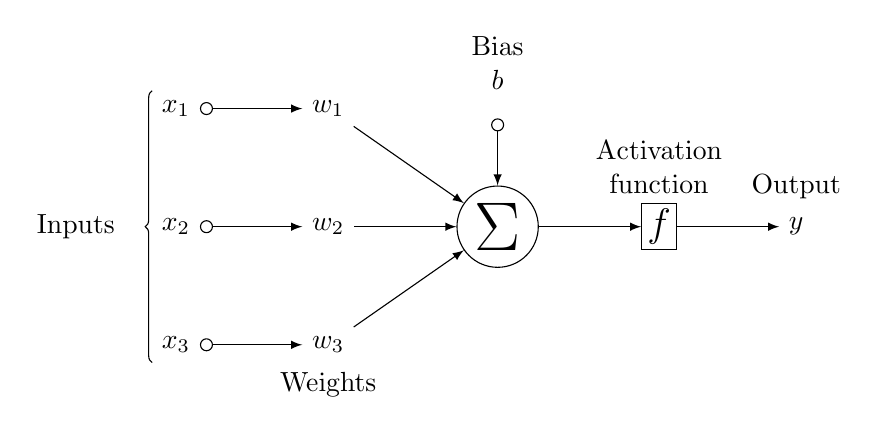
\begin{tikzpicture}[
init/.style={
  draw,
  circle,
  inner sep=2pt,
  font=\Huge,
  join = by -latex
},
squa/.style={
  draw,
  inner sep=2pt,
  font=\Large,
  join = by -latex
},
start chain=2,node distance=13mm
]
\node[on chain=2] 
  (x2) {$x_2$};
\node[on chain=2,join=by o-latex] 
  {$w_2$};
\node[on chain=2,init] (sigma) 
  {$\displaystyle\Sigma$};
\node[on chain=2,squa,label=above:{\parbox{2cm}{\centering Activation \\ function}}]   
  {$f$};
\node[on chain=2,label=above:Output,join=by -latex] 
  {$y$};
\begin{scope}[start chain=1]
\node[on chain=1] at (0,1.5cm) 
  (x1) {$x_1$};
\node[on chain=1,join=by o-latex] 
  (w1) {$w_1$};
\end{scope}
\begin{scope}[start chain=3]
\node[on chain=3] at (0,-1.5cm) 
  (x3) {$x_3$};
\node[on chain=3,label=below:Weights,join=by o-latex] 
  (w3) {$w_3$};
\end{scope}
\node[label=above:\parbox{2cm}{\centering Bias \\ $b$}] at (sigma|-w1) (b) {};

\draw[-latex] (w1) -- (sigma);
\draw[-latex] (w3) -- (sigma);
\draw[o-latex] (b) -- (sigma);

\draw[decorate,decoration={brace,mirror}] (x1.north west) -- node[left=10pt] {Inputs} (x3.south west);
\end{tikzpicture}
\caption{Artificial Neuron Diagram}
\end{figure}
An artificial neuron is an approximate mathematical model of a biological neuron, and is intended to fulfill similar purposes. Each artificial neuron has multiple inputs from other neurons. Along with the inputs, each neuron has a weight for each input, a bias term, and activation function, and only one output. The output of one neuron travels to other neurons and becomes of their inputs. The output of a neuron is expressed mathematically for $n$ inputs $x$ and weights $w$, a bias term $b$, and activation function $f(x)$ as follows:


$$activation = \sum\limits_{i=0}^n x_i w_i+b$$
$$output = f(activation)$$

Mentioned above, weights are positive or negative numbers which scale the effect or relevance of their accompanying inputs on a neuron's single output. Besides the weights, another important component of a neuron is the activation function, whose primary is to transform the output of a neuron. Common activation functions include a sigmoid curve, a hyperbolic tangent, a binary step function, and a rectifier function.The sigmoid activation and hyperbolic tangent activation functions are often used for general purpose neural networks due to their gradient nature, fixed range, and the fact that they are easily differentiated. Finally, the bias term is a number added to the summation of weighted inputs, which allows us to make transformations on the domain of the activation function.
\begin{figure}[h]
\centering
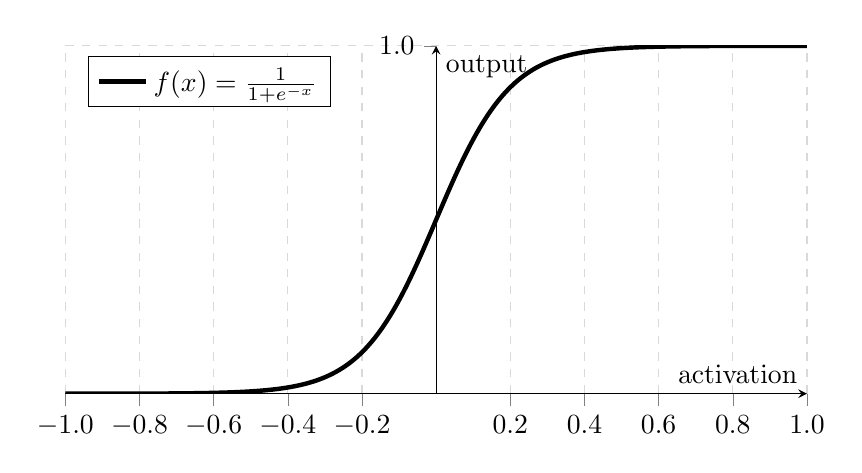
\begin{tikzpicture}
    \begin{axis}[
    	legend pos=north west,
        axis x line=middle,
        axis y line=middle,
        ytick={0,1},
        x tick label style={/pgf/number format/fixed,
                            /pgf/number format/fixed zerofill,
                            /pgf/number format/precision=1},
        y tick label style={/pgf/number format/fixed,
                            /pgf/number format/fixed zerofill,
                            /pgf/number format/precision=1},
        grid = major,
        width=11cm,
        height=6cm,
        grid style={dashed, gray!30},
        xmin=-1,     % start the diagram at this x-coordinate
        xmax= 1,    % end   the diagram at this x-coordinate
        ymin= 0,     % start the diagram at this y-coordinate
        ymax= 1,   % end   the diagram at this y-coordinate
        %axis background/.style={fill=white},
        xlabel=activation,
        ylabel=output,
        tick align=outside,
        enlargelimits=false]
      % plot the stirling-formulae
      \addplot[domain=-1:1, black, ultra thick,samples=500] {1/(1+e^(-10*x))};
      \addlegendentry{$f(x)=\frac{1}{1+e^{-x}}$}
    \end{axis}
\end{tikzpicture}
\caption{Sigmoid Function Graph}
\end{figure}
\subsubsection{Feed-forward Neural Network}
Constellation utilizes a feed-forward neural network, a collection of neurons organized into layers, as classifying mechanism for detection various features in a image. In a feed-forward neural network, the output of each neuron is the input of each neuron in the next layer. In this manner, the original inputs of the network are "fed forward" to new neurons in new layers, passing through a number of hidden layers in the middle, and finishing at the output layer.The outputs of the neurons in the final layer (output layer) are the outputs of the whole network and are used to judge the conclusion the network made.
\subsubsection{Backpropagation}
%\begin{figure}[h]
\centering
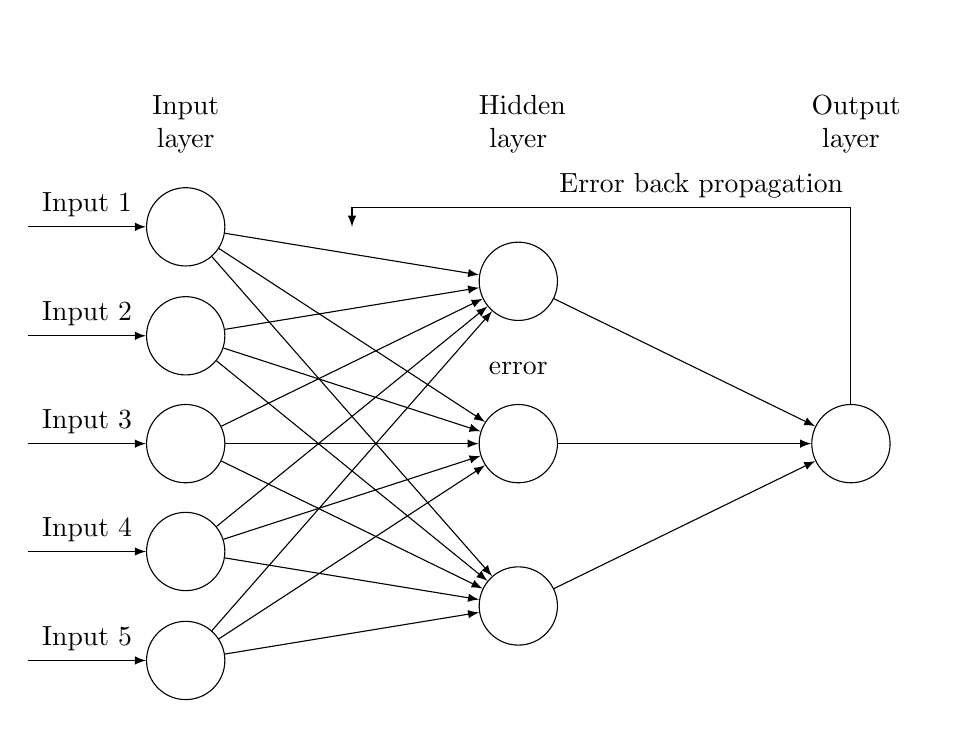
\begin{tikzpicture}[
    plain/.style={
      draw=none,
      fill=none,
      },
    net/.style={
      matrix of nodes,
     nodes={
       draw,
        circle,
    inner sep=10pt
    },
  nodes in empty cells,
  column sep=2cm,
  row sep=-9pt
  }, 
 >=latex
 ]
\matrix[net] (mat)
{ 
|[plain]| \parbox{1cm}{\centering Input\\layer} & |[plain]| \parbox{1cm}{\centering     Hidden\\layer} & |[plain]| \parbox{1cm}{\centering Output\\layer} \\
& |[plain]| \\
|[plain]| & \\
& |[plain]| \\
|[plain]| & |[plain]| \\
& & \\
|[plain]| & |[plain]| \\
& |[plain]| \\
|[plain]| & \\
& |[plain]| \\
};
\foreach \ai [count=\mi ]in {2,4,...,10}
  \draw[<-] (mat-\ai-1) -- node[above] {Input \mi} +(-2cm,0);
\foreach \ai in {2,4,...,10}
{\foreach \aii in {3,6,9}
  \draw[->] (mat-\ai-1) -- (mat-\aii-2);
}
\foreach \ai in {3,6,9}
  \draw[->] (mat-\ai-2) -- (mat-6-3);
%\draw[->] (mat-6-3) -- node[above] {Ouput} +(2cm,0);
\path [line] node{error} -- (mat-1-1);
\draw[->] (mat-6-3) -- ++(0pt,3cm) -| node[pos=0.15,above] {Error back propagation} ( $ (mat-2-1)!0.5!(mat-2-2) $ );
\end{tikzpicture}
\caption{A Feed-Forward Neural Network}
\end{figure} 

Supervised learning is the process of adjusting the weights of each neuron in a neural network in an effort to reach target outputs from a specific set of inputs, effectively "fine tuning" the neural network to make it as correct as possible. One of the most common methods of adjusting a neural network's weights is called backpropagation, first developed in Werbos in 1974.
\begin{figure}[h]
\centering
\tikzset{every picture/.style={line width=0.75pt}} %set default line width to 0.75pt        

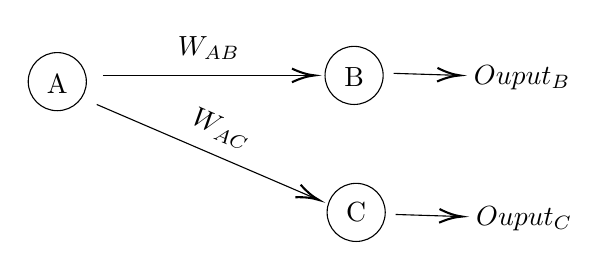
\begin{tikzpicture}[x=0.75pt,y=0.75pt,yscale=-1,xscale=1]
%uncomment if require: \path (0,300); %set diagram left start at 0, and has height of 300

\draw    (111, 74) circle [x radius= 14, y radius= 14]  ;
\draw    (130,85) -- (235.16,130.21) ;
\draw [shift={(237,131)}, rotate = 203.26] [color={rgb, 255:red, 0; green, 0; blue, 0 }  ][line width=0.75]    (10.93,-3.29) .. controls (6.95,-1.4) and (3.31,-0.3) .. (0,0) .. controls (3.31,0.3) and (6.95,1.4) .. (10.93,3.29)   ;

\draw    (255, 137) circle [x radius= 14, y radius= 14]  ;
\draw    (133,71) -- (233,71) ;
\draw [shift={(235,71)}, rotate = 180] [color={rgb, 255:red, 0; green, 0; blue, 0 }  ][line width=0.75]    (10.93,-3.29) .. controls (6.95,-1.4) and (3.31,-0.3) .. (0,0) .. controls (3.31,0.3) and (6.95,1.4) .. (10.93,3.29)   ;

\draw    (254, 71) circle [x radius= 14, y radius= 14]  ;
\draw    (273,70) -- (303,70.94) ;
\draw [shift={(305,71)}, rotate = 181.79] [color={rgb, 255:red, 0; green, 0; blue, 0 }  ][line width=0.75]    (10.93,-3.29) .. controls (6.95,-1.4) and (3.31,-0.3) .. (0,0) .. controls (3.31,0.3) and (6.95,1.4) .. (10.93,3.29)   ;

\draw    (274,138) -- (304,138.94) ;
\draw [shift={(306,139)}, rotate = 181.79] [color={rgb, 255:red, 0; green, 0; blue, 0 }  ][line width=0.75]    (10.93,-3.29) .. controls (6.95,-1.4) and (3.31,-0.3) .. (0,0) .. controls (3.31,0.3) and (6.95,1.4) .. (10.93,3.29)   ;


\draw (111,75) node  [align=left] {A};
\draw (255,137) node  [align=left] {C};
\draw (254,72) node  [align=left] {B};
\draw (184,58) node   {$W_{AB}$};
\draw (190,97) node [rotate=-23.81]  {$W_{AC}$};
\draw (335,72) node   {$Ouput_{B}$};
\draw (336,140) node   {$Ouput_{C}$};


\end{tikzpicture}
\caption{Single Branch of a Backpropagation Neural Network}
\end{figure}
In order to train neural networks through backpropagation (BP), we use examples. Each set of example inputs, known as training sets, are connected to a target output, which the system is aware of, and together the two parts form a training pair. The first step of training a BP network is to pass the training set through the neural network with randomly generated weights. The error, represented as $\delta$, for an output neuron is the difference between the actual output and the target output for that training set. Consider the abbreviated neural network illustrated in Figure 4. Assume this network has only an input layer consisting of an unspecified number of input neurons with unspecified outputs, a hidden layer containing only Neuron $A$, and an output layer consisting of Neurons $B$ and $C$. Obviously, $W_{AB}$ and $W_{AC}$ are the weights of the edges connecting the neurons. We complete the backpropagation action by modifying weight $W_{AB}$, replacing it with $W^+_{AB}$, as follows:
$$\delta_B=Target_B-Output_B$$
$$W^+_{AB}=W_{AB}+(\delta_B\times Output_A)$$

This approach is what is also used to adjust the weight of Neuron $C$ from the example. This approach, however, cannot calculate more appropriate weights for neurons whose outputs feed into the inputs for another neuron, referred to as hidden layer neurons, such as neuron $A$, because there is no predefined and confirmed target value. Therefore, we must calculate the error of the output of $A$ indirectly by backpropagating from the output layer neurons, whose errors have already been calculated. For $A$, this could be shown as:
$$\delta_A = (W_{AB}\times\delta_B)+(W_{AC}\times\delta_C)$$

Once we have established the error for Neuron $A$, its updated weights can be calculated with the same approach used for $B$ and $C$. This pattern is used throughout the full neural network to calculate the adjusted weights for hidden layers in order to converge upon the network's target output.
\begin{figure}[h]
\centering
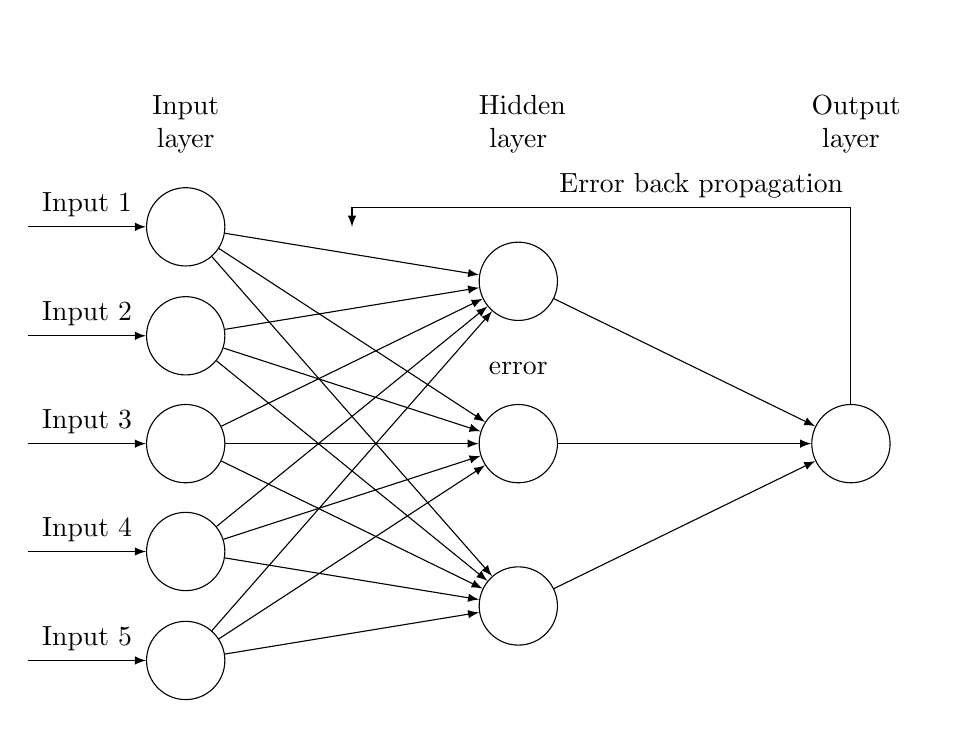
\begin{tikzpicture}[
    plain/.style={
      draw=none,
      fill=none,
      },
    net/.style={
      matrix of nodes,
     nodes={
       draw,
        circle,
    inner sep=10pt
    },
  nodes in empty cells,
  column sep=2cm,
  row sep=-9pt
  }, 
 >=latex
 ]
\matrix[net] (mat)
{ 
|[plain]| \parbox{1cm}{\centering Input\\layer} & |[plain]| \parbox{1cm}{\centering     Hidden\\layer} & |[plain]| \parbox{1cm}{\centering Output\\layer} \\
& |[plain]| \\
|[plain]| & \\
& |[plain]| \\
|[plain]| & |[plain]| \\
& & \\
|[plain]| & |[plain]| \\
& |[plain]| \\
|[plain]| & \\
& |[plain]| \\
};
\foreach \ai [count=\mi ]in {2,4,...,10}
  \draw[<-] (mat-\ai-1) -- node[above] {Input \mi} +(-2cm,0);
\foreach \ai in {2,4,...,10}
{\foreach \aii in {3,6,9}
  \draw[->] (mat-\ai-1) -- (mat-\aii-2);
}
\foreach \ai in {3,6,9}
  \draw[->] (mat-\ai-2) -- (mat-6-3);
%\draw[->] (mat-6-3) -- node[above] {Ouput} +(2cm,0);
\path [line] node{error} -- (mat-1-1);
\draw[->] (mat-6-3) -- ++(0pt,3cm) -| node[pos=0.15,above] {Error back propagation} ( $ (mat-2-1)!0.5!(mat-2-2) $ );
\end{tikzpicture}
\caption{A Feed-Forward Neural Network}
\end{figure} 

%% The Appendices part is started with the command \appendix;
%% appendix sections are then done as normal sections
%% \appendix

%% \section{}
%% \label{}

%% References
%%
%% Following citation commands can be used in the body text:
%% Usage of \cite is as follows:
%%   \cite{key}          ==>>  [#]
%%   \cite[chap. 2]{key} ==>>  [#, chap. 2]
%%   \citet{key}         ==>>  Author [#]

%% References with bibTeX database:

%%\bibliographystyle{model1-num-names}
%%\bibliography{sample.bib}

%% Authors are advised to submit their bibtex database files. They are
%% requested to list a bibtex style file in the manuscript if they do
%% not want to use model1-num-names.bst.

%% References without bibTeX database:

% \begin{thebibliography}{00}

%% \bibitem must have the following form:
%%   \bibitem{key}...
%%

% \bibitem{}

% \end{thebibliography}


\end{document}

%%
%% End of file `elsarticle-template-1-num.tex'.